% The document class supplies options to control rendering of some standard
% features in the result.  The goal is for uniform style, so some attention 
% to detail is *vital* with all fields.  Each field (i.e., text inside the
% curly braces below, so the MEng text inside {MEng} for instance) should 
% take into account the following:
%
% - author name       should be formatted as "FirstName LastName"
%   (not "Initial LastName" for example),
% - supervisor name   should be formatted as "Title FirstName LastName"
%   (where Title is "Dr." or "Prof." for example),
% - degree programme  should be "BSc", "MEng", "MSci", "MSc" or "PhD",
% - dissertation title should be correctly capitalised (plus you can have
%   an optional sub-title if appropriate, or leave this field blank),
% - dissertation type should be formatted as one of the following:
%   * for the MEng degree programme either "enterprise" or "research" to
%     reflect the stream,
%   * for the MSc  degree programme "$X/Y/Z$" for a project deemed to be
%     X%, Y% and Z% of type I, II and III.
% - year              should be formatted as a 4-digit year of submission
%   (so 2014 rather than the accademic year, say 2013/14 say).

\documentclass[ % the name of the author
                    author={Gavin Parker},
                % the name of the supervisor
                supervisor={Dr. Neill Campbell},
                % the degree programme
                    degree={MEng},
                % the dissertation    title (which cannot be blank)
                     title={Deep Siamese Networks for Illumination Estimation from Stereo Images},
                % the dissertation subtitle (which can    be blank)
                  subtitle={},
                % the dissertation     type
                      type={research},
                % the year of submission
                      year={2018} ]{dissertation}

\begin{document}
% =============================================================================

% This macro creates the standard UoB title page by using information drawn
% from the document class (meaning it is vital you select the correct degree 
% title and so on).

\maketitle

% After the title page (which is a special case in that it is not numbered)
% comes the front matter or preliminaries; this macro signals the start of
% such content, meaning the pages are numbered with Roman numerals.

\frontmatter

% This macro creates the standard UoB declaration; on the printed hard-copy,
% this must be physically signed by the author in the space indicated.

\makedecl

% LaTeX automatically generates a table of contents, plus associated lists 
% of figures, tables and algorithms.  The former is a compulsory part of the
% dissertation, but if you do not require the latter they can be suppressed
% by simply commenting out the associated macro.

\tableofcontents
%\listoffigures
%\listoftables
%\listofalgorithms
%\lstlistoflistings

% The following sections are part of the front matter, but are not generated
% automatically by LaTeX; the use of \chapter* means they are not numbered.

% -----------------------------------------------------------------------------

\chapter*{Executive Summary}

\noindent
In this paper we present a system for estimating the lighting in photographs and video streams of real scenes, that improves on previous work by eliminating the need for explicit geometry estimation or reflectance mapping steps. We make use of similar features in stereo views of an object to construct a lighting prediction without the need for known geometry, which can then be used to render superimposed objects with realistic illumination parameters.
\newline
Augmented Reality is a growing topic in computer graphics and vision, that involves superimposing synthetic information and images on real scenes, often with the aim of giving the illusion that the object is part of the real world. Current AR solutions use geometry estimation to correctly place and scale the virtual objects to fit into the real scene, but do very little to render those objects with other scene intrinsics. Our system uses a Siamese Convolutional Neural Network to extract the lighting intensities and directions from objects within a scene, such that virtual objects can be re-rendered with realistic lighting parameters on-the-fly.

The appearance of an object is made up of its material properties, its geometry and the lighting conditions, making estimation of any one of these factors from a single image a difficult task. Previous work has tackled lighting estimation by treating geometry estimation as a separate problem, making use of depth cameras or known geometry. This has a significant performance penalty, and estimated surface normals are often too noisy to be useful. I have produced a CNN that relies on the relative invariance of these 3 unknowns with respect to time, by attempting to predict illumination from a series of views of an object. By using a Siamese approach, with shared weights, the Neural Network is able to identify similar features \todo{/position?} in multiple views of the scene, and infer geometry. This represents an improvement in practicality over the previous work and takes the technique a step closer to being deployed on mobile devices.

\begin{quote}
My research hypothesis is that a siamese CNN provided with RGB stereo images, can predict a light probe at an object without the need for explicit geometry estimation or the use of a depth camera.
\end{quote}

To test my hypothesis I performed research and implementation as follows:

\noindent
\begin{itemize}
\item Researched existing algorithms and neural network architectures for lighting and geometry estimation.
\item Replicated the work of Stamatios Georgoulis et al. by building CNNs that can interpolate sparse reflectance maps and predict environment map lighting from single objects with provided geometry.
\item Implemented a dataset generator that could produce realistic lighting parameters and images for training networks.
\item Created a new siamese architecture to encode geometry from stereo images and estimate lighting conditions.
\item Assessed the quality of these networks with a suite of image similarity benchmarks.
\end{itemize}

Our network is able to achieve equivalent results to previous work, predicting lighting from an object with unknown geometry and material from stereo images or video frames.
\chapter*{Supporting Technologies}

{\bf A compulsory section, of at most $1$ page}
\vspace{1cm} 
\begin{quote}
\noindent
\begin{itemize}
\item Tensorflow was used to construct and train deep learning models.
\item OpenCV libraries were used for image parsing and manipulation in experiments and final models.
\item Blender was used to evaluate the quality of produced HDRIs, and to create scenes for training data.
\item HDRIHaven was used as a source of ground truth environment maps.
\item Shapenet was used for example 3D model data for experiments.
\item OpenEXR was used in experiments to parse Radiance HDR image data.
\item Cycles renderer was used to produce photorealistic synthetic data.
\item IKEA Dataset was used to train the final suite of models.
\end{itemize}
\end{quote}

% -----------------------------------------------------------------------------

\chapter*{Notation and Acronyms}

{\bf An optional section, of roughly $1$ or $2$ pages}
\vspace{1cm} 


\begin{quote}
\noindent
\begin{tabular}{lcl}
AR                 &:     & Augmented Reality                                         	\\
CNN                 &:     & Convolutional Neural Network                             	\\
HDR					&:		& High Dynamic Range										\\
SSIM				&:		& Structural Similarity										\\
sRGB				&:		& standard Reg Green Blue									\\
BR(S)DF				&:		& Bidirectional Reflectance(Scattering) Distribution Function
\end{tabular}
\end{quote}

% -----------------------------------------------------------------------------

\chapter*{Acknowledgements}

{\bf An optional section, of at most $1$ page}
\vspace{1cm} 

\noindent
% It is common practice (although totally optional) to acknowledge any
%third-party advice, contribution or influence you have found useful
%during your work.  Examples include support from friends or family, 
%the input of your Supervisor and/or Advisor, external organisations 
%or persons who  have supplied resources of some kind (e.g., funding, 
%dvice or time), and so on.

% =============================================================================

% After the front matter comes a number of chapters; under each chapter,
% sections, subsections and even subsubsections are permissible.  The
% pages in this part are numbered with Arabic numerals.  Note that:
%
% - A reference point can be marked using \label{XXX}, and then later
%   referred to via \ref{XXX}; for example Chapter\ref{chap:context}.
% - The chapters are presented here in one file; this can become hard
%   to manage.  An alternative is to save the content in seprate files
%   the use \input{XXX} to import it, which acts like the #include
%   directive in C.

\mainmatter

% -----------------------------------------------------------------------------

\chapter{Contextual Background}
\label{chap:context}

{\bf A compulsory chapter,     of roughly $5$ pages}
\vspace{1cm} 
\section{Computer Graphics and Lighting}

\noindent
Traditional computer graphics involves creating virtual scenes, with geometry represented as a series of surfaces in 3D space. Each surface is given properties such as texture and material, and virtual lights are placed in the scene with given intensities and colors. Given the position and size of a virtual camera images can be produced by calculating the resultant color at every point on a the screen, produced by a combination of the lighting and surface properties. This can be achieved through Raytracing which involves simulating the paths of all light rays that meet the camera within the scene. While physically accurate this is a slow process that is impractical for real-time rendering. In real-time rendering tasks a process called Rasterisation is used, where the geometry is culled so that only surfaces in view of the camera need to be considered. This, in combination with lighting and material approximations, makes it possible for convincing characters and objects to be rendered at 60 frames per second.
\todo{Maybe unnecessary}
The material of a surface defines how it reflects or absorbs incoming light, and as a result characterizes its colour under different lighting conditions. In the physical world, no surface is perfectly even on a microscopic scale. When an incoming photon reaches a surface, its angle of reflection is actually dictated by the shape collides with, making per-photon reflections very difficult to predict even for very smooth surfaces. Furthermore many photons are actually absorbed by the material depending on it's colour properties and the lights wavelength. However, visible light is made up of a vast supply of photons, which can even be considered as a wave with properties like wavelength or amplitude. If we consider light on a macroscopic scale it is far easier to predict and represent. We often use the concept of 'colour' to refer to the wavelengths of light which an object reflects, where lighter objects reflect more wavelengths and darker objects reflect fewer and absorb more photons. It is essential to note that the colour something takes on is actually representative of the wavelengths of light that it reflects towards the light sensing device, be it an eye or a camera. Very smooth objects such as mirrors reflect most wavelengths, at very predictable angles, and so take on different colours depending on the viewpoint. These behaviours are captured in the 'Rendering Equation', 
\[L_0(x, w_0, lambda) = L_e(x, w_0, lambda) + \int_{ohm}{f_r(x, w_i, w_o,lambda)L_i(x, w_i, lambda)dw_i}\],
 \todo{Simplify this}
which Computer Graphics attempts to approximate.
\newline
In Computer Graphics, materials are often referred to as having 'Diffuse' and 'Specular' properties, which capture the aforementioned behaviour. This is in fact an approximation that allows for the efficient rendering of surfaces, though does not capture the light behaviour perfectly. 'Diffuse' refers to the wavelength, or colour, of light that is reflected off a surface equally in every direction. This can be thought of as the 'base colour', that is somewhat invariant to the viewpoint of the observer. A material that is entirely diffuse is often reffered to as 'Lambertian'. 'Specularity' refers to how reflective an object is, and is often used to approximate the light being reflected directly from a light source towards the observer. The 'Phong Shading' model combines these two elements to roughly represent a variety of materials, under the assumption that reflective materials have a dominant component that can be modelled as a mirror. For example an unlaquered wooden panel will be very unreflective and may contain no 'specular' component at all as its colour remains fairly consistent when observed from every direction. On the other hand a plastic ball will have a dominant colour but also reflect a lot of the incoming light, which is modelled as a combination of the incoming light direction and the surface angle. Modern Raytracing makes use of a far more accurate model called a Bidirectional Reflectance Distribution Function, which defines a probability distribution function. This function gives the probablity of an incoming photon with angle of incidence i, reflecting with an angle of incidence j. Over many photons this is able to accurately capture the reflective behaviour of a surface, and is often used in combination with properties like 'Albedo' and 'Subsurface Scattering' to result in an almost photorealistic surface.
\begin{center}
\begin{figure}
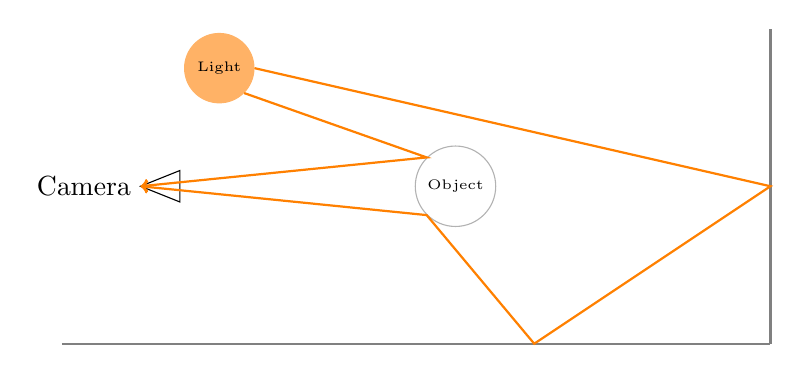
\begin{tikzpicture}
\draw[gray, thick] (-1,0) -- (8,0); %floor
\draw[gray, thick] (8,0) -- (8,4); % wall
\node[draw, circle, minimum size=1cm, draw=gray!60] at (4,2) (obj){\tiny Object};
\node[draw, circle, minimum size=5mm, draw=orange!60, fill=orange!60] at (1,3.5) (sun){\tiny Light};
\draw[black] (0,2) -- (0.5,2.2) -- (0.5,1.8) -- cycle node[anchor=east] {Camera}; % camera
\draw[->,orange,thick] (sun.south east) -- (obj.north west) -- (0,2); %direct ray
\draw[->,orange,thick] (sun.east) -- (8,2) -- (5,0) -- (obj.south west) -- (0,2); %indirect ray


\end{tikzpicture}
\label{raytracing}
\caption{The direct illumination is a combination of the light source properties and the object material. The indirect ray is a combination of the light source properties and the material of all the surfaces it collides with}
\end{figure}
\end{center}
A product of the reflective nature of surfaces results in 'indirect lighting', an effect that is extremely difficult to capture in real-time rendering. The incoming light on a surface is made of photons arriving directly from light sources as well as photons being reflected from other surfaces, as demonstrated in \ref{raytracing}. Often when rendering is expensive it is appropriate to approximate the lighting in the scene to contain only 'direct' and 'environment' lighting. In this approximation, all objects are lit by the environment light, which represents an approximate light in all directions at all points in the scene. This is very cheap to render, as provided there is no direct lighting, all points on a surface recieve a constant amount of light. Direct lighting refers to lighting objects based on their proximimity to a given light source, ignoring shadows that would require calculating and intersections between the light and the surface. Unfortunately this approximation results in very unconvincing images as in reality the light at a point is made up of all the photons being reflected from that point. The Phong shading model ignores the effect of photons being reflected many times within a scene, and so misses much of the subtle detail. A common way of calculating indirect lighting is 'Global Illumination', which involves tracing the paths of many light rays from light sources as they are reflected within the scene. To save computation is is often performed in reverse, where rays are drawn from the camera and reflected a constant number of times. The illumination of the final reflection is then computed from the direct lighting, which is then passed between the reflected surfaces to achieve the approximate lighting at the original scene point. This is a very expensive procedure and innapropriate for real-time rendering, where other approximations can be used. One such approximation is an 'Environment Map' or 'Environment Probe', which is the precomputed representation of all the incident light at a single point. This can be thought of as a panorama image at a single point, capturing both the direct and indirect light, as shown in \ref{environment map}. While this cannot be used for every point in the scene, it is fair to assume that nearby objects have similar incident lighting. A common application is to use a large environment map to represent the lighting in outdoor scenes, where the main light source is the sky. This results in a vast improvement over a single Environment/Direct light combination, while still being inexpensive to compute. Furthermore, multiple environment maps can be blended together to roughly represent the lighting across larger scenes, often in combination with other approximations such as baked lighting.
\newline
A benefit of 'Environment Maps' is that rather than being computed, they can be captured from real-world data. This is a technique often used in films to apply the lighting from a set to virtual additions. This is achieved by taking photographs of a reflective sphere under different exposures to capture a range of lighting intensities. These images can then be composited to capture the range of light in a single format. By using a sphere, which has known geometry, it is easy to invert the image into a High Dynamic Range panorama. It is essential to use an HDR format, as RGB captures only a very narrow range of light intensity.
\begin{center}
\begin{figure}
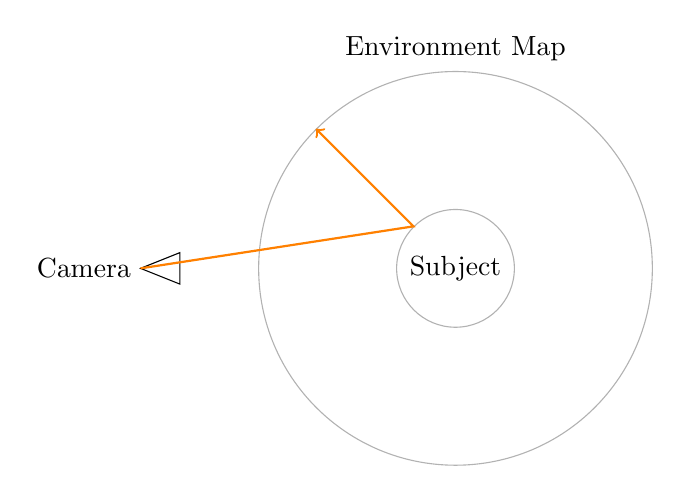
\begin{tikzpicture}
\node[draw, circle, minimum size=5cm, draw=gray!60] at (4,2) (env){};
\node[above] at (env.north) {Environment Map};
\node[draw, circle, minimum size=1cm, draw=gray!60] at (4,2) (obj){Subject};

\draw[black] (0,2) -- (0.5,2.2) -- (0.5,1.8) -- cycle node[anchor=east] {Camera}; % camera
\draw[->,orange,thick] (0,2) -- (obj.north west) -- (env.north west); %direct ray


\end{tikzpicture}
\label{environment map}
\caption{An environment map being used to render a sphere to the camera. This process is reversed with a perfectly reflective sphere to obtain the environment map}
\end{figure}
\end{center}
\section{Augmented Reality}
Augmented Reality is an extension of computer graphics, where virtual objects are rendered on a real video stream to appear as if they are part of the original scene. This creates additional challenges as many of the parameters that are used in computer graphics are not available. While the material and geometry of the added objects is known, the geometry and lighting of the real scene must either be estimated, or manually recorded beforehand. The latter option tends to be used in films, where the layout of the scene and camera movements are known beforehand. In this case the geometry of the scene can be measured and recreated in 3D modelling or CAD software for a virtual approximation. Similarly, the lighting at points in the scene can be captured using a light probe, often a reflective sphere, and taking composite photographs at different exposures. This process results in an 'Environment Map' which captures the color and intensity of all the incoming light at a single point. With this data, additional characters can be rendered entirely in the virtual space, interacting with the approximated geometry and being lit by blended combinations of light probes across the scene. Provided that the virtual camera moves exactly as the real camera, the added object can be masked and overlaid onto the original video of the scene. To aid this process it is possible to estimate a cameras motion by tracking the movement of stationary markers within the camera view.
\newline
In live AR, as is becomming common in mobile applications, the scene data must be approximated entirely from data gathered from the devices sensors. Geometry estimation is performed using a process known as Salient Localization and Matching, which can be used to track the movement of a camera through a 3d environment. SLAM relies on finding similar points from multiple camera views, with the assumption that these points share the same position in 3D space. Given known camera parameters such as focal length, and the relative position of the cameras between the views, it is then possible to triangulate these salient points to find their location. SLAM is used extensively in the field of robotics, often using stereo cameras such that scene points can be calculated at every frame of an incoming video stream. By tracking the movement of 3D points in a video, it is not only possible to track the cameras movements, but to also build a 3D mapping of the scene geometry. In the context of AR it is essential to track the cameras position as it corresponds to the users position within the Mixed Reality environment. Furthermore by building a 3d map of the environment it is possible to find appropriate surafces on which to place virtual objects, or even apply shadows.
\newline
Another scene parameter that must be estimated is the lighting. Unlike geometry estimation which has significant uses in the field of robotics, solutions for lighting estimation tend to be more rudimentary. For real-time estimation, especially on mobile devices, it is common to simply pick the fastest approximation to maximise performance. In fact, mobile graphics hardware is far less powerful than what is used in the film industry, meaning that even perfect lighting representations may result in an unrealistic image. Nonetheless, mobile graphics hardware continues to improve and the quality bottleneck for AR will eventually shift to lighting estimation. In the case of shadows and reflective objects, good lighting estimation is a necessity. One fast approach is to simply take an intensity average across each incoming video frame, and use this to determine the overall brightness of the image. This is very approximate, and ignores light direction and colour but means that superimposed objects do not appear overly bright in dark areas and visa versa. There are also some techniques that make use of machine learning to estimate incoming light direction given some basic constraints light a single light source (usually outside), which restricts the possible incoming light or strictly portrait images, which reduce the possible scene geometry and materials.
\newline
The difficulty of these tasks arises from the fact that lighting, material and geometry are linked unknown parameters, and so an understanding of one is required to estimate the other. For example a red sphere may appear so because it is painted red, or because it is reflective and the lighting of the scene is red in tone. In fact this problem is the basis for many optical illusions, as it is sometimes difficult for humans to determine what exactly they are seeing under certain conditions. Humans share most of the properties of a moving mobile AR device, yet are able to infer properties of the environment under most circumstances. We achieve this by making assumptions and approximations while also utilising prior knowledge and a semantic understanding of the world around us. It is these features that we must formalise and exploit if we are to build convincing AR tools.
\newline
One feature that humans and computer vision sytems can exploit is shadows, where the light from a light source is blocked from reaching it's destination. In the case that we have an object of consistent shape and material such as a flat table, it is sensible to treat significantly darker patches on the surface as shadows. If we can find the object that is casting the shadow, it can be trivial to triangulate the light source. However, this technique is only accurate if there are no invariances in lighting across the scene that could result in changes in brighness across surfaces without explicit shadows. This model is still useful however, especially in outdoor scenes where we can treat the sun as a single light source, approximately equidistant from every point in the scene. In this case, any darkening on objects of the same material must be caused by shadowing. In indoor scenes we cannot make this assumption; often there are multiple light sources, which are close enough to the objects in the scene to cause differences in direct lighting. However in indoor scenes we have other consistencies to benefit from such as more uniform geometry. When we consider indoor scenarios, especially those likely to be applicable to AR and film we find that there are regular flat surfaces such as floors and furniture that are reasonably consistent in geometry. While the assumption that the light source is infinitely far away doesn't apply here, we are able to restrict light sources to likely directions, such as artificial light from bulbs above or natural light from windows. While these assumptions can aid in lighting prediction, it is still extremely difficult to build a robust lighting estimation system for indoor scenes, resulting in the simplified techniques used in todays AR platforms.
\newline
Often the reason humans find it easy to understand the light in a scene is because of a semantic understanding. While we do not know the geometry of every room we enter, we are able to recognise consistencies that we have encountered before. While a single image patch could technically be any combination of material, light and geometry we can restrict the likely combinations by recollecting previous times we have seen something similar. We understand, for example that surfaces with dramatic variances in color and light intensity are more likely to be a reflective metal than to have those diffuse colour properties. Similarly if we see an orange tinted outdoor scene we know to assume that it is probably due to the color of the sky, because we recognise that known surfaces like grass or concrete are not naturally that colour.
\section{Machine Learning and Artificial Intelligence}
Because the complicated nature of semantics it is very difficult to create a system that explicitly relies on finding known patterns between scenes to cover all cases. For example it would be viable to create a system tht extracts IKEA furniture from scenes, and uses the known geometry and material to treat the furniture as sparse light probes. This would not be able to account for scenes without known furniture, outdoor scenes or even scenes where the furniture is partially obscured. Instead it is a sensible approach to consider machine learning. Machine Learning is a field of Computer Science that involves training the parameters of a system on data to make predictions. By taking known input and output pairs it is possible to adjust the parameters of the system such that it can generalise to inputs with unknown outputs. In our case it would be possible to train a model to take input images, either raw or preprocessed, and output some representation of the lighting. Traditional ML models such as the Support Vector Machine are able to learn a given number of parameters from some input features. These features could be extracted from the image, such as the average intensity or the dominant frequency in the foutier domain. These models are easy to train and can produce very predictable results, but require the designer to explicitly provide a set of features that they believe can be used to seprerate or define the different outputs. For example if our task was to predict whether a given image was 'indoors' or 'outdoors' we have restricted our problem to binary classification - our outputs are known. It would then be feasible to provide some features, such as average colour or number of colour clusters above a threshold to then train an SVM.
\newline
If we wish to predict a more complicated lighting model we must be able to take into account many more features than what we can feasibly define by hand. In this case we can look to the field of AI, and explicitly Convolutional Neural Networks. In the field of AI it is possible to train a model without explicit features, by using an approximation of neural dynamics in real brains. In broad terms, we programmatically create a series of connected neurons in a layered structure, with each neuron having a number of inputs and some number of outputs. The neurons have a very simple behaviour - they multiply each input by some 'weight' and provide the accumulated result as the output.
\[y_k = \sum_{j=0}^{m}{w_{kj}x_j}\]
By training on known results we can adjust these weights so that the final neuron layer (which matches our desired output data shape) contains the desired output.
\newline
Convolutional Neural Networks are a recent development in AI that allows for reasonably fast AI models that take images as input. Rather than having a neuron for each colour of each pixel, we can instead learn the weightings for a 'convolution'. A convolution, in this context, is a function which can be passed across an image to extract features,
\[\sum_{n_1=-s}^{s}{\sum_{n_2=-s}^{s}{f[n_1, n_2]\cdot g[x-n_1,y-n_2]}} \]
and often resembles a SxS matrix. Convolutions are used frequently in computer vision, as they are an efficient way of computing many popular image features such as Harris Corners or Sobel edges. In a CNN we intend to learn the weights of many convolutional matrices to quickly extract featured from the input image. Furthermore we are able to pass further convolutions across the results from previous convolutional layers to learn more complex features. For example the first layer could extract edges while a second layer extracts the presence of 'X' shapes. CNNs make it possible to train deep and complex models on image data, resulting in robust models that often vastly outperform their traditional ML counterparts.
\newline
The performance of CNNs is heavily impacted by the choice of metrics used to decide the weights and behaviour for each neuron. When given inputs and weights a neuron may or not fire depending on an 'activation function'. In biological neurons, this is a complex nonlinearity that is difficult to efficiently capture in artificial neural networks. Instead we use approximations like 'Relu',
\[f(x) = log(1 + e^x),\]
to decide whether to fire after calculating the output value. Furthermore during training it is important to consider how to adjust the weights to converge on the optimum. For this we use a 'Loss Function', which computes an error value given the desired, or ground truth, value and our models prediction. The rate of change of this erroris then used to iteratively adjust the weights of each neron based on its influence.
\newline
 The prime application of CNNs has been in image classification, where the model must distinguish between a set number of classes. However it is possible to use CNNs for regression tasks that output other images using the concept of 'deconvolutional' layers. These learn an interpolation matrix that increases the dimensionality of the input. Popular image regression architectures often involve a series of convolutional layers followed by a series of deconvolutional layers. The aim of the convolutional layers is to learn a deep representation of the content of the image, often removing the original spatial dimension. Rather than 'shallow' features like edges or colours, these features ideally represent som 'understanding' of the scene such as presence of some object or shape of the environment. The deconvolutional layers can then interpolate this data into a new image that will often share many common features with the original. For example in style transfer, the convolutional layers attempt to extract the content of the image while the deconvolutional layers interpolate the image features with weights representing some artistic style.
\newline
The difficulty in the application of CNNs often lies in the 'training' stage; while a deep enough network should be able to learn a mapping for any function, the difficulty in providing data to capture every case increases with the problem complexity. If a network is trained to recognize images of dogs, it will only be able to learn features from dogs that it has seen as input. As a result, if a new dog is provided that lacks some of the features of the training data, it may be missclassified. Regression tasks in particular attempt to learn a complex funtion and so need a vast amount of training data to be able to generalise. This becomes problematic where the training data is hard to collect and classify. In the case of image classification, many photographs can be taken and marked with their intended class. With image regression this can become an extremely laborious task as the desired output needs to be extracted by hand. Often there are large datasets already available that can help speed up the process, especially if the datasets are labelled, or if features can be extracted by hand. However it is simply necessary to manually create a dataset to train a network to face a new task. Fortunately there are still some steps that can be taken to accelerate this process, such as data augmentation. This usually involves manipulating some training inputs in such a way as to introduce variances while maintaining the classification, and can greatly increase the amount of data available. Another approach is to create synthetic virtual data, by rendering new images. It is important to note however that the synthetic data must be accurate enough such that a model trained on it can generalise to real world data. It is often sensible to mix real world and synthetic data when training a model for the best results.


% -----------------------------------------------------------------------------

\chapter{Technical Background}
\label{chap:technical}
\section{Commercial Lighting Solutions}
Lighting solutions in the film\&TV industry tend to involve precalculating or precapturing the lighting in a scene before adding virtual characters. In the film 'I,Robot', Digital Domain \footcite{https://www.digitaldomain.com/work/i-robot/} \todo{Better references for this commercial stuff} created a semi-automated system for capturing HDR environment maps using a rotating fisheye-lens camera. Once placed, the camera was able to take shots at multiple angles and at a range of exposures, before compositing the shots together to produce a usable HDR lighting map. Often these HDR maps are not used in isolation, but along with footage of a proxy for the virtual addition, so the filmmakers can qualitatively measure how the materials react with the set lighting. These techniques allow filmmakers to capture an approximation of lighting with limited camera equipment and makes it easier to create complex panning and dolly shots of scenes with real and virtual elements, which would otherwise require a green-screen. Over time, camera equipment has become more advanced and it is faster to take high quality shots at multiple exposures. As a result, later films such as 'The Curious Case of Benjamin Button' are able to utilise multiple lighting probes to illuminate characters. By taking lighting samples across the scene, virtual characters can then be lit partly according to their position in the world by blending environment maps together. This creates a more convincing final render as the approximate indirect lighting from nearby objects becomes more apparent. The downside of these hollywood techniques is that the lighting data must be captured beforehand for every environment used. This is a long, laborious and expensive process as the cameras required to take accurate shots at different exposures need to be extremely accurate to produce correct composites. It is also important to note that compositing images is difficult and also requires human input to match black levels, tones and camera properties that are hard to automate.
\newline
Recent commercial AR platforms do contain some level of lighting estimation from input video data. Apple's ARKit is able to estimate the colour and intensity of the ambient lighting in some scenes \footcite{https://developer.apple.com/documentation/arkit/arlightestimate}, by analyzing the pixels of the incoming video frame. This technique adds some realism to AR applications, as objects can be dimmed or brightened with the scene, so as not to stand out. However this is a very rough estimate of lighting, and contains no directional information or approximation of indirect illumination  Google's ARCore has similar functionality, taking an average of the luminance values across the video to estimate the intensity \footcite{https://developers.google.com/ar/reference/unity/prefab/Environmental_Light}. It is possible to estimate the light direction from a face tracking scene however, by using the tracked face as a light probe \footcite{https://developer.apple.com/documentation/arkit/ardirectionallightestimate}. By using a face, the application is able to restrict the possible lighting scenearios to a range of likely geometries and materials that make up human faces. The platform is able to produce not only the primary light direction and intensity, but also an approximation of the environment lighting as spherical harmonics. While incredibly useful for some application such as the retouching of portrail photographs, the technique is not robust to different scenes as it relies on the approximation of some known geometry.
\newline
Upcoming AR applications are experimenting with new methods of integrating the scene lighting with virtual augmentations. Magic Leap is making use of tailored hardware called a 'Light Field' camera, which involves the use of an array of microlenses to capture additional information from the scene. Each microlens is able to capture information from multiple camera points, so that extra depth and lighting information can be extracted from the frame. This is a significant improvement on IR depth cameras such as the Microsoft Kinect, which can't be used outside. By extracting depth, and therefore surface geometry information, it is far easier to reason about the reflectance of objects within the scene and estimate the lighting. However, light-field cameras are extremely expensive and inpractical for mobile AR. Most mobile devices contain normal high quality cameras as well as accurate intertia sensors, which can be used in combination with stereo matching for a similar depth estimation model.
\section{Lighting Estimation Research}
Early techniques for lighting estimation were able to find the direction of a single primary light source, under significant constraints. In \footcite{http://ieeexplore.ieee.org/stamp/stamp.jsp?tp=&arnumber=990650}, Peter Nillius and Jan-Olof Eklundh were able to estimate a single light direction, provided the input image contained an appropriate lambertian surface. By making use of an 'occluding contour' it is possible to infer some detail of the geometry, as the surface of the visible edge of a contour that occludes itself will always be perpendicular to the view direction of the observer. Using the lambertian lighting model, along with the edge intensity it is possible to make a prediction using a bayesian network for the incoming light direction. This is a simple method that exploits inherent properties of real geometry, but has too many prerequisites to be practical. While it captures direction, it also ignores colour, intensity and any indirect lighting. 
\todo{More basic stuff here}
In \cite{Lalonde-2009-10350}, Lalonde et al. are able to estimate a more complete set of parameters for environmental lighting from single outdoor photographs. By segmenting the image into sky, ground and vertical surfaces, and extracting features like shadows, the authors are able to reliable predict the sun's position. While very robust for outdoor applications, this approach does not consider light intensity or colour. Furthermore, the reliance on outdoor scenes restricts its usage in AR.
Scott Wehrwein et al. demonstrate a technique for sun direction and shadow detection from multiple input images \cite{http://www.cs.cornell.edu/projects/shadows/files/wehrwein_3dv15_shadows.pdf}. They use illumination rations to extract shadows, after constructing a sparse 3D representation of the scene from stereo matching of multiple images. By exploiting shadow boundaries on the derived surface normals, it is then possible to determine the light direction. This work shows how multiple views can be used to infer knowledge of the geometry of the scene, to make the problem of lighting estimation more constrained. However, like previous work it assumes a perfectly lambertian surface and clear outside conditions, restricting the possible lighting conditions significantly.
\newline
It is clear that estimating a full representation of the illumination within a scene is very difficult given the number of unknowns. However predicting only the direct light sources is still very valuable, as this makes up the majority of the light within a scene, and can be combined with image colour values to give an approximation of the indirect lighting. Shadows are a good indicator of the direction and intensity of direct lighting. They not only give some indication of direction based on shape, but also the intensity through the contrast of colour values between areas that are shaded and unshaded. Takahiro et al. demonstrate techniques for recovering illumination from shadows in \footcite{http://ieeexplore.ieee.org/stamp/stamp.jsp?tp=&arnumber=1315013}. This work compares two methods, \textit{Spherical Harmonics} and \textit{Haar Wavelets} for estimating the illumination from cast shadows on known geometry. Spherical Harmonics are function defined over a whole sphere, and are useful for defining the light reflectance at a point, as in Global Illumination. The work demonstrates how this method fails to capture higher frequency illumination values, and presents \textit{Haar Wavelets} as an alternative. This method is able to approximate functions as a series of linear combinations of Haar functions, and is able to more efficiently capture a higher range of light frequencies at a point. \todo{Read more on this, spherical harmonics appear a lot}
\newline
An interesting approach from Microsoft Research \footcite{http://www.cs.wm.edu/~ppeers/showPublication.php?id=Xia:2016:RSS} attempts to reconstruct the shape and reflectance of an object from a video with known motion and camera pose. This is achieved by decoupling the estimation of geometry from the estimation of illumination, and refining initial estimates over a series of video frames. While the lighting is not known in the scene, the camera pose and motion must be known and so this work is only applicable under carefully controlled environents. However it effectively demonstrates how multiple views of an object can be used to refine predictions of scene understanding, under the reasonable assumptions of static lighting, material and per-object geometry.
\newline
An emerging trend in lighting estimation research is the use of 'light fields' as a way of representing the light on an entire scene. A light field represents the radiance of light flowing in each direction in each point in space, resulting in a 5D function. Capturing and storing light field data is difficult as for a given area, light must be sampled in all directions at all points, which is impractical using traditional cameras. The use of microlens light-field cameras, which sample incoming light rays at a range of angles, has made capturing light-fields much less costly, resulting in datasets becoming available such as that of \footcite{http://hazirbas.com/datasets/ddff12scene/}. Light fields require immense quantities of storage capacity and contain far more light information than is required in the field of AR, making their use inpractical. Instead most work has been centered around the estimation of light at a single point, either at the camera view or in the scene, that can be seen as a sparse sampling from the light-field.
\footcite{http://ieeexplore.ieee.org/stamp/stamp.jsp?tp=&arnumber=790313}
\todo{Talk about CNNs for estimating geometry/material}
\section{Machine Learning for scene understanding}
To calculate the lighting of a scene, some assumptions or approximations must be made about the material or geometry to constrain the problem. It is therefore important to consider previous techniques to extract these features from images, especially geometry estimation which has significant applications in the field of robotics. In 2015, David Eigen et al. demonstrated a CNN approach to estimate depth, surface normals and semantic labels from single input images \footcite{https://arxiv.org/pdf/1411.4734.pdf}. Here they use a 'multi-scale' architecture, where outputs from early features passed as input to later deconvolutional layers, as well as subsequent convolutional layers. Multi-scale features can often lead to faster inference as important features are 'short-circuited' closer to the output, reducing the need for large deep layers at inference time \todo{Citation needed ;) }. The results of this work are extremely promising, and suggest that a single RGB image may be enough to infer a complex understanding of the scene. If it is possible to understand variations in the illumination and material in a scene to find geometry then it follows that it is possible to understand geometry and material to find illumination.  However the network shown is very deep and trained primarily on indoor scenes. Its use in the field of AR is limited, as the hardware is much more limited in terms of GPU resources. Furthermore while the network is able to predict depth and surface normals on a large scale, successfully finding walls and floors, it struggles with more complex geometry.
\newline
There has been some work in inverse lighting specifically for the rendering of AR objects, notably that of \footcite{https://link.springer.com/content/pdf/10.1007/s00371-010-0501-7.pdf}. In this work the user must simply provide a ping-pong ball, representative of a lambertian sphere, while the least-squares algorithm is performed on the lighting equation, using features of the sphere as constraints. This results in an approximation of illumination as a series of point lights and spherical harmonoics which can practically be used for rendering. The downside however is that the process of presenting the system with a known ball can take upwards of 20 seconds, and the resultant lighting is suitable for only primarily diffuse objects. This does however demonstrate how powerful even basic knownledge of the geometry and material of the scene can be for deriving the lighting.
\section{Machine Learning for Illumination Estimation}
Most of the previous worhttp://hazirbas.com/datasets/ddff12scene/k has had to rely on significant assumptions for the scene to constrain the lighting to fit known phenomena, that can be exploited to estimate the illumination. It is clear that due to the unconstrained nature of the problem, that some assumptions about geometry, material and lighting must be made. Rather than making the required assumptions to fit a model, another approach is building a model to find and exploit assumptions from real data using machine learning. Given enough scene features and data it is possible to learn approximations and assumptions to produce a more robust model. In \footcite{https://arxiv.org/pdf/1611.06403.pdf}, Yannick Hold-Geoffroy et al. use a CNN-based technique to estimate sky parameters from outdoor photographs to a high enough degree of accuracy that virtual objects can be re-rendered. In this work, the output illumination model is constrained to the Hosek-Wilkie model with parameters representing the sun position, ground albedo and light wavelength. A dataset is then constructed by selecting small LDR sections of real HDR scene panoramas, resulting in a large number of sample photographs, and HDR lighting ground-truths. This work demonstrates extraordinary performance, but is limited in output format by the lighting model which is constrained to outdoor images with clear skies. This ignores the indirect lighting from scene objects and indoor scenes, but demonstrates how CNNs with the right data can be used to exploit more subtle image features to predict lighting.
\newline
There have been advancements in the field towards estimating the lighting in indoor scenes, such as that by \footcite{https://arxiv.org/pdf/1704.00090.pdf}. In this work, Gardner et al. use a very large dataset of indoor HDRI environment maps to train a CNN to predict the environment map at the cameras position. This environment map can then be warped to provide an approximate environment map for a given position. The resulting network is very accurate for predicting light direction and intensity, but fails to predict colours which must be provided for a user. Furthermore the network is very deep, making it difficult to deploy on mobile devices. While the warping operator user is innovative, it fails to accurately capture the lighting at points in 3d space, and instead provides a rough approximation.
\section{Predicting Light Probes}
CNNs can exploit different features in a scene to determine lighting such as shadows or object reflectance. One example that uses the latter is 'Deep Reflectance Maps' \footcite{https://arxiv.org/pdf/1511.04384.pdf} by Konstantinos Rematas et al. In this work it is demonstrated that better accuracy can be achieved by constraining the CNN input to a specific feature, in this case a sparse reflectance map, provided the geometry is known. By taking the brightest pixel for every surface normal on an object, a sparse representation of it's reflectance can be built and fed to a CNN for interpolation. This work makes use of a large synthetic dataset but still results in good performance on real world data, allowing the researchers to then modify the shape of specular virtual objects while still maintaing a realistic surface appearance. An important feature of this work is that the researchers present results from reflectance maps produced from perfect surface normals, and from those produced by noisy estimated normals. It is demonstrated that the estimated normals are unsuitable for accurate reflectance mapping, and actually result in poorer predictions than a direct appearance-to-lighting network.
\newline
This work was then extended for illumination estimation in 'What is Around the Camera', by using a precalculated sparse reflectance map in combination with a segmented background image. In this work, a full HDR environment map is predicted to a degree of accuracy that allows the superimposition of rendered geometry with fairly accurate lighting. Both of these works use a Convolutional-Deconvolutional approach to produce a new image as output. The limitations of this work however are due to required prior calculations rather than restrictive assumptions about the scene. While the network can handle objects of multiple materials, they must be segmented and seperate sparse RMs calculated. Furthermore the calculation of the sparse RM relies upon knowledge of the surface normals of the object being used. The researchers point to previous work \todo{Talk about this} on the usage of CNNs for surface normal and depth estimation but fail to demonstrate the accuracy of their work with these more noisy estimated surface normals. It is also apparent that there is significant data loss in the calculation of the sparse reflectance map, which makes significant assumptions about the object in question, ignoring the effects of shadows and how lighting changes based on both position and surface orientation.
\newline
These works demonstrate that if surface geometry is known, a network can be trained to accurately reproduce lighting conditions, using an object as a probe. However they point to 2 significant shortcomings that we attempt to address in this work. Firstly the use of sparse reflectance maps in isolation ignores a significant amount of useful information on the object that could be used to estimate the lighting. As a result, a direct approach of predicting illumination from a single image view can often outperform cases where the reflectance map is too sparse or the material is very diffuse. Secondly, modern surface normal estimation techniques from single images are not accurate enough to constrain the problem of lighting estimation. We believe that the use of a network that exploits multiple views of an object, provided the scene parameters remain constant, will be able to more accurately predict the geometry through learned stereo matching. Furthermore, a network that simultaneously learns geometry and lighting will be able to exploit more scene features such as shadows, that would otherwise be unavailable in an explicit reflectance mapping.
\newline
\begin{figure}
\def\checkmark{\tikz\fill[scale=0.4](0,.35) -- (.25,0) -- (1,.7) -- (.25,.15) -- cycle;} 
\begin{tabular}{|c|c|c|c|c|}
Model & Known Geometry & Known Material & Direct Lighting & Indirect Lighting \\
Mirror Ball & \checkmark & \checkmark & \checkmark & \checkmark \\


\end{tabular}
\caption{Summary of current methods}
\end{figure}

% -----------------------------------------------------------------------------

\chapter{Project Execution}
\label{chap:execution}

{\bf A topic-specific chapter, of roughly $15$ pages} 
\vspace{1cm} 

\section{Reproducing Prior Art in Tensorflow}
\begin{wrapfigure}{r}{0.6\textwidth}
\centering
\begin{tikzpicture}
\node[rectangle, minimum size=4cm, anchor=north, draw=black!60](encode) {};
\node[below] at (encode.north) {Encode Block};
\node[rectangle, minimum size=2.5cm, draw=black!60, below=5mm of encode.north](loop) {};
\node[rectangle, draw=black!60, below=3mm of loop.north](conv) {Convolution};
\node[rectangle, draw=black!60, below=3mm of conv.south](bn) {Batch Norm};
\node[rectangle, draw=black!60, below=3mm of bn.south](relu) {Relu};
\node[rectangle, draw=black!60, below=2mm of loop.south](mp) {Max Pooling};
\node[right] at (loop.east) {$\times N$};

\end{tikzpicture}

\caption{An Encode Block}
\label{encode}
\end{wrapfigure}
It was important to reproduce the preceeding work, to assess its aplicability in the field of AR and create a fair benchmark for evaluating our new models and approach. We began with a reimplementation of 'Deep Reflectance Maps', a recent work that demonstrated promising results from a CNN based approach. This work was a necessary prerequisite to 'What is around the Camera?', which demonstrates how the reflectance map of an object can be extracted and used to predict it's lighting. The project was provided with a dataset for replication, but without any source code. Fortunately the architecture was well documented and so easily reproduced in a modern deep learning framework. For this work I used Tensorflow, a python deep learning framework that gave me the flexibility to add unique network features such as a reflectance mapping step, as well as export the model to different platforms.

\begin{center}
\begin{figure}
\begin{tikzpicture}[
network/.style={rectangle,draw=green!50,fill=green!5, thick, minimum height=4cm},
layer/.style={rectangle, draw=black!50,anchor=center},
]
\node[](Normals){\includegraphics[width=2cm]{images/normals_1}};
\node[below=of Normals]	(Appearance){\includegraphics[width=2cm]{images/appearance_1}};
\node[rectangle, draw=red!50,fill=red!5, thick, text width=1cm](RM)[below right =0.5cm of Normals, above right =0.5cm of Appearance] {RM};
\node[right=0.5cm of RM]	(Sparse RM){\includegraphics[width=2cm]{images/sparse_rm_1}};

\node[network, minimum width=3cm] (CNN)  [right=0.5cm of Sparse RM]{};
\node[layer, below=3mm of CNN.north, minimum width=2cm] (conv_1) {128};
\node[layer, below=5mm of conv_1.south, minimum width=1cm] (conv_2) {32};
\node[layer, below=5mm of conv_2.south, minimum width=0.75cm] (conv_3) {16};
\node[layer, below=5mm of conv_3.south, minimum width=0.5cm] (conv_4) {8};

\node[network, minimum width=3cm,draw=red!50,fill=red!5] (DCNN)  [right=0.5cm of CNN]{};
\node[layer, below=7mm of DCNN.north, minimum width=1cm] (deconv_2) {32};
\node[layer, below=7mm of deconv_2.south, minimum width=0.75cm] (deconv_3) {16};
\node[layer, below=7mm of deconv_3.south, minimum width=0.5cm] (deconv_4) {8};

\node[right=of DCNN]	(Reflectance){\includegraphics[width=2cm]{images/gt_lighting_1_warped}};

\node[above=2mm of CNN.north, opacity=0](a){};
\node[below=2mm of CNN.south, opacity=0](b){};
\node[above=2mm of DCNN.north, opacity=0](c){};

\draw[->] (Normals.east) -| (RM.west);
\draw[->] (Appearance.east) -| (RM.west);
\draw[->] (RM.east) -- (Sparse RM.west);
\draw[->] (Sparse RM.east) |- (a.center) -- (CNN.north);
\draw[->] (CNN.south) -- (b.center) -| (DCNN.south);
\draw[->] (DCNN.north) -- (c.center) -| (Reflectance.west);

\end{tikzpicture}
\caption{Deep Reflectance Maps - Combine known (or inferred) surface normals to form a sparse reflectance map. A series of Convolutional layers is followed by a series of Deconvolutional layers to estimate a dense RM. Each layer is followed by batch normalization, max pooling and the Relu activation function.}
\end{figure}
\end{center}

The network in question is a Convolutional-Deconvolutional network trained to produce dense reflectance maps from single sparse reflectance maps as input. The training data was provided as the segmented image of an object, in this case a Shapenet car, and surface normals. It was necessary to first construct a system for extracting a sparse reflectance map from these inputs according to the approximation stated in the work. A reflectance map is a map from every surface normal to a luminance value, and can be thought of as the appearance of a material on a perfect gaussian sphere. In this case each point on the sphere has a unique surface normal, with no possibility for self-shading. In the case of the Shapenet car, there are many repetitions of the same surface normal, often with different illuminations, as well as some missing surface normals altogether. We build a sparse representation map,
\[ R_i = max(n\cdot n_i \cdot L)\],
where the reflectance R, at angle i on the gauss sphere is the maximum illumination, L, of all pixels sharing i in the original image. It is important to note that we only consider a half-sphere as surface facing away from the camera are naturally occuded. Also some information is lost by taking a maximum illumination, as we make the rough assumption that any darker pixels with the same surface orientation must be due to self-shading. This is the case as we are modelling the target in question as a point object, with all lights infinitely far away, which is the approximation being made with the use of Environment Maps.
\newline
The process for calculating the reflectance is mathematically intensive, but can be represented in a graph form as
\begin{algorithm}
$ diffs \leftarrow sphere \times input^T $\;
$ reflectance \leftarrow mask(intensity, diffs > \cos(0.0872665)) $\;
$ indices \leftarrow argmax(reflectance) $\;
$ reflectance_map \leftarrow colour[indices] $\;
\end{algorithm}
using matrix multiplication and boolean masks. This was initially implemented sqequentially in the numpy maths package as a proof-of-concept but was too slow to operate on the number of training samples required. By migrating the implementation to use native tensorflow operations, the per-batch runtime was reduced from 6 seconds to 20ms, making it feasible to use during training.
\newline
The network architecture was fairly simple, consisting of 'encode' blocks made up of convolutional layers, followed by batch normalization, max pooling and the relu activation funcction. In each block the convolutions were repeated a given number of iterations, with only the max-pooling step changing the dimensionality of the tensor, as shown in \ref{encode}. These 'encode' blocks were also used in all subsequent models for feature extraction. This was easy to implement in Tensorflow, leaving most of the time for training and optimizing the process. Due to the quantity of training data provided (50,000 samples) it was necessary to pipeline the input data stream to make best use of the hardware resources available on BlueCrystal4. By using a pipeline, it is possible to use the CPU for preprocessing operations such as data conversion and image resizing, leaving the GPU for the more intensive training process. This resulted in much faster training and allowed for a larger batch size than was used in the previous work. The model was trained for 50 epochs to produce results of similar quality to the original. Furthermore it was possible to compare the results to an end-to-end implementation which only used the original images as input. Suprisingly the results were very similar, with the end-to-end approach sometimes even outperforming the refectance mapped version. The reason for this was the assumption of good quality surface normals. If ground truth surface normals are used, the reflectance mapped version vastly outperforms the others. Unfortunately, even CNN based methods for estimating surface normals from single images are fragile and result in very noisy estimates.
\todo{Diagram of these results?}
\newline
During the implementation of the previous work, I constructed wrapper functions to use as building blocks to quickly construct 'encode' and 'decode' layers for future networks. This made implementing the 'What is behind the camera?' network far easier. This work was provided with both the original dataset of synthetic and real images, as well as source code. However the source code was provided for the 'MatConvNet' matlab library, which was slow, lacked documentation and unavailable on many platforms. As such I thought it beneficial to also reproduce this work in Tensorflow, using many of the utilities created for the last model. This network is very similar, taking a sparse reflectance map, along with a segmented background, as input and producing a High Dynamic Range environment map as output.
\newline
Unfortunately this task presented difficulties in data formatting that resulted in poor training until they were resolved. Firstly to encourage the network to extract luminance, the input data was first converted to CiE LAB colour space using a Tensorflow utility from the 'Pix2Pix' network \footcite{https://github.com/affinelayer/pix2pix-tensorflow/blob/master/pix2pix.py}. While the conversion proved accurate for the traditional RGB color inputs, it was unable to convert HDR formatted images, in this case the ground truth environment map. This is due to how HDR images are stored, to capture a larger range of light intensities thatn RGB. For this task we used the Radiance RGBE file format, which is simpler than the OpenEXR alternative \todo{give an example}. The data is stored as RGB values with an exponent, but interpreted in python as floating point RGB values with a very large range. This data needed to be formatted in such as was as to reduce the range to 0,1 whithout data loss. After experimenting with different ways of formatting the data I decided to use a logarithmic representation, after shifting the values to be above 1. In this format I was able to fully reconstruct the original HDR image, and the LAB space outputs of my network could also be converted into HDR without any loss of quality.
\newline
The original work consisted of two models, one that used single material objects and one that used segmented multi-material objects. The multi-material network was a very simple improvement on the original, where the object was first segmented into 3 materials, and fed as input to 3 identical convolutional networks. The output of these convolutions was then concatenated and fed into the deconvolutional step to again produce a single HDR environment map. As I was able to achieve good results with the single material network, I thought it was unnecessary to also train the multi-material model, which effectively provided a denser reflectance map to the network. I trained over 50 epochs, each consisting of 56,000 samples, with a learning rate of 1.6e-9. The output to this architecture was a 64x64 HDR environment map that could then be imported into graphics software for qualitative analysis. Being such a low resolution, it bared little structural resembles to the original full resolution environment map. It did however appear to be a good approximation of the low-resolution version, and would result in very reasonable lighting when used as an HDRI to render objects, when compared to the original. It was found that the quality of the approximation depended heavily on the density of the provided reflectance map, and the complexity of the lighting in the scene. In cases where the scene was outside, even with very sparse reflectance maps, the network was able to infer features such as sky and ground colour as well as approximate sun position. This was due to the simplicity of the scene lighting, leading to cases where the lighting conditions could be adequately approximated almost entirely from the background image. Some indoor scene, especially those containing a mix of synthetic lights and windows resulted in very poor predictions. In these scenes, very dense reflectance maps had to be provided to produce good results. \todo{Put some images here}
\newline
It is important to note that while these results were promising, they were based on reflectance maps obtained using perfect surface normals, limiting their use in practical applications. 
\section{Stereo Model Architecture}
It was apparent from the results of the previous work that the sparse reflectance map and background combination was not enough data to construct a robust model for both indoor and outdoor scenes. By explicitly calculating the reflectance, ignoring shadow information and assuming point-like objects, much of the appearance data is removed. Furthermore the surface normal calculation required is impractical from a single image, due to the unconstrained nature of an object's appearance. Instead of relying on explicit reflectance maps, we took a new approach to design models that could exploit the additional spatial information of stereo images to infer surface normals, allowing the network to learn it's own model of reflectance. While this approach requires more information (multiple images), this information is available in use cases such as AR and film editing. One consideration was to simply use a stereo matching technique to calculate a relative depth map from the stereo images and find the surface normals. These estimated normals could then be used in the previous network to estimate the environment lighting. However stereo matching is a difficult task that often involves human intervention, and does in fact rely on extracting identical convolutional features from the two images and finding their spatial differences. Most stereo matching techniques are slow, and while they can produce a good estimate of the depth of objects in a scene, they cannot produce surface normals to the degree of accuracy we require. Instead we construct a model based on learned stereo matching, providing the model with two views of an object, allowing it to learn an internal representation of geometry and lighting. By using two views, provided to two sets of convolutional layers, before being combined in intermediate layers, the network can extract similar features and exploit consistencies between views. To this end we also present results from a 'siamese' network, where the weights in the convolutional layers are shared, such that the same features are extracted from each view. We also present a network that simultaneously estimates object geometry along with the scene lighting.
\newline
For our prediction task we make the following assumptions:
\begin{itemize}
\item Provided objects consist of a single material with constant albedo. Materials can contain Diffuse, Specular and Subsurface properties.
\item Geometry and lighting remain static between both stereo views.
\item Stereo view distance is kept constant, though object size can vary. Views are also parallel.
\item Subjects are modelled as floating objects. In the use-case where lighting on a surface is required, the surface lighting can be composited onto the light probe trivially.
\item Camera intrinsics are kept constant.
\end{itemize}
The previous work was adapted to a siamese network by sharing weights between the convolutional layers. The two inputs are fed into two identical 'Encode' blocks, consisting of a number of convolutional layers with batch normalization and max pooling. However, during the training psrocess, only the weights for the first path are trained. These weights are duplicated in the second path to ensure that the same convolutions are being performed on each image of the pair. The output of these two paths is then concatenated before being passed into the deconvolutional steps. Multi-scale features are also used, passing features for the second path into the deconvolutional layers. An important difference in this network is that we do not provide the network an explicit background image, in fact the resolution of the background is lowered to give a depth-of-field effect. In real stereo images, the background would also move with the camera, however capturing this data is impractical. Fortunately due to the parallax effect, the background appears to move far less than the foreground anyway and so this approximation does not cause significant issues. The model was trained with similar parameters to the previous network, using a L1 loss function on the predicted and ground truth environment map.
\section{Dataset Creation}
The most difficult part of many deep learning tasks, including this one, is the creation of an unbiased and generalised dataset. For the purposes of this task we needed a large dataset of stereo image pairs accompanied by an HDR environment map. Capturing this data in the wild is a very laborious process, and requires expensive camera equipment. Instead I took the more practical approach of generating and utilizing synthetic data, which presents its own set of unique problems. For this task we make use of the open source 3D modelling program 'Blender' and the accompanying raytracer 'Cycles'. This made it possible to create photo-accurate renders with realistic lighting and materials. The data must be accurate in terms of lighting, material and geometry if the model is to be able to generalise to real world scenarios. To ensure accurate geometry we used the IKEA dataset \footcite{http://ikea.csail.mit.edu/} of 3D models, which includes a large range of furniture accurately modelled. The objects represent a good analogue for real geometry one might find in scenes, with some objects self-occluding and self shadowing. The models contained a mix of flat surfaces, edges and curves although being furniture the dataset contained a bias towards flat surfaces. We believe this is reasonable however, as most scenes in AR applications and films will be dominated by flat surfaces such as floors and walls.
\newline
To introduce further variance into the dataset, we make sure to apply different materials to the furniture to represent the range of materials found in real scenes. It is important that these materials react realistically to the lighting in the scene, rather than relying on explicitly lambertian surfaces. For this task we make use of Blender's 'Principled BSDF' shader \footcite{https://docs.blender.org/manual/en/dev/render/cycles/nodes/types/shaders/principled.html}, referred to as an 'Uber' shader for it's ability to represent any range of materials. Bidirectional Scaterring Distribution Functions are able to accurately simulate the reflection of light on a surface, and by varying parameters such as albedo colour, reflectiveness and subsurface scattering we are able to approximate a range of real materials. While most surfaces can be represented using this shader, our dataset generator does contain some restrictions. Notably, while we vary material properties and colour, we do not apply texture to the object, so the subtle variations that can be seen in materials like cloth or carbon fibre are not simulated. However we believe that in most cases these subtleties are not visible due to the quality of the input video stream from AR platforms and do not have a significant in the overall reflective properties of most surfaces.
\newline
To generate our ground truth environments, and to light the objects we use HDRI images taken from \footcite{https://hdrihaven.com/}. These environment maps are used as both backgrounds and light sources by blender to illuminate the provided objects. These HDRI images are captured from real environments and are claimed to be accurately colour corrected. To further augment the dataset and prevent overfitting we introduce random rotation. For each stereo pair we load a random model from our dataset, apply a random material and select a random environment. We then move our virtual camera to a random orientation, within a reasonable range, facing the target object. We also re-render the environment map to have it's forward direction aligned with that of the observer camera. \todo{Probably a diagram of this stuff} This prevents the network from simply learning to select from our modest set of HDRIs, and instead encourages it to learn to extract the environment entirely from the input. This generator was used to produce 55,000 image sets, making use of 28-core intel processors on the Blue Crystal 4 supercomputer. After experimentaiton, it was found that due to the small image sizes and work distribution of path tracing, that high core-count CPUs outperformed the GPU renderer implementation.

\begin{figure}[h]
\centering
\begin{tabular}{| c | c | c | c |}
\includegraphics[width=3cm]{images/left/0} &
\includegraphics[width=3cm]{images/right/0} &
\includegraphics[width=3cm]{images/normals/0} &
\includegraphics[width=3cm]{images/hdri/0.png} \\
\includegraphics[width=3cm]{images/left/11} &
\includegraphics[width=3cm]{images/right/11} &
\includegraphics[width=3cm]{images/normals/11} &
\includegraphics[width=3cm]{images/hdri/11.png} \\
\includegraphics[width=3cm]{images/left/22} &
\includegraphics[width=3cm]{images/right/22} &
\includegraphics[width=3cm]{images/normals/22} &
\includegraphics[width=3cm]{images/hdri/22.png} \\
\end{tabular}
\caption{Generated data examples - Left, Right, Surface Normals, Environment Map (Tonemapped to RGB)}
\label{data_examples}
\end{figure}
\section{Experiments}
To assess the accuracy and performance of the models, I set up a series of experiments on the same training and test data set. I trained the Siamese Stereo model for 100 epochs, with a learning rate of 1.7e-9, and evaulated predictions on 1000 test samples. I repeated this step for the same model without the siamese shared weights, and for the original 'What is around the Camera?' work.

\chapter{Critical Evaluation}
\label{chap:evaluation}

\section{Model Accuracy}
To evaluate the accuracy of the models we use a suite of image comparison measures on the produced HDRI environment maps. It is essential that the metrics used suitably evaulate the image similarity, and so we consider which image properties are most influential of the resulting lighting. The most basic estimation should be able to capture the direction and intensity of direct lights within the scene. Often there are few direct lights, but their effect on lighting dominates the overall scene illumination. Better predictions will be able to capture some information on indirect lighting, such as sky or wall colour and brightness.
\todo{Talk a bit more about this}
\newline 
We start with two basic difference metrics, the L1 and L2 norm, which are both per-pixel Minkowski distances. These measures are fast to calculate and simple to implement and so are often used as the loss function in image regression tasks. L2 norm involves the squaring of pixel differences, and exagerrates the effect of large pixel differences on the overall similarity score. In the HDR domain this can mean that direct lights, such as the sun, which are predicted to be in a slightly different direction, will have a severe impact on the similarity, despite having a minor effect on the resulting illumination. When we inspect light sources in sRGB photographs, it appears as if the light source is large and emmitting light from a radius, as the higher brightness values fall outside of the cameras exposure bracket. \ref{rgb_example} demonstrates this effect, as parts of the woman's face, as well as the surrounding sky have the same colour values as the center of the sun, as the camera fails to capture the brightness rage. A minor misprediction in sun position here will have little effect on the L2 distance, but in HDR would have a significant impact.
\newline
Another commonly used image comparison metric is the SSIM \footcite{http://ieeexplore.ieee.org/stamp/stamp.jsp?tp=&arnumber=1284395},
\[SSIM(x,y) = \frac{(2u_xu_y + c_1)(2\sigma_{xy} + c_2)}{(u^2_x + u^2_y + c_1)(\sigma^2_x + \sigma^2_y + c_2)}\]
which aims to predict the accuracy of an image with human perception. It is a measure of structure, which takes luminance and contrast into account, and so many be better suited for HDR. Finally, we assess the models ability to identify the direction of the provailing light source, by taking the spherical distance between the brightest pixel in the ground truth and predicted image.
\todo{Put a table of results here followed by discussion}

\begin{figure}[h]
\centering
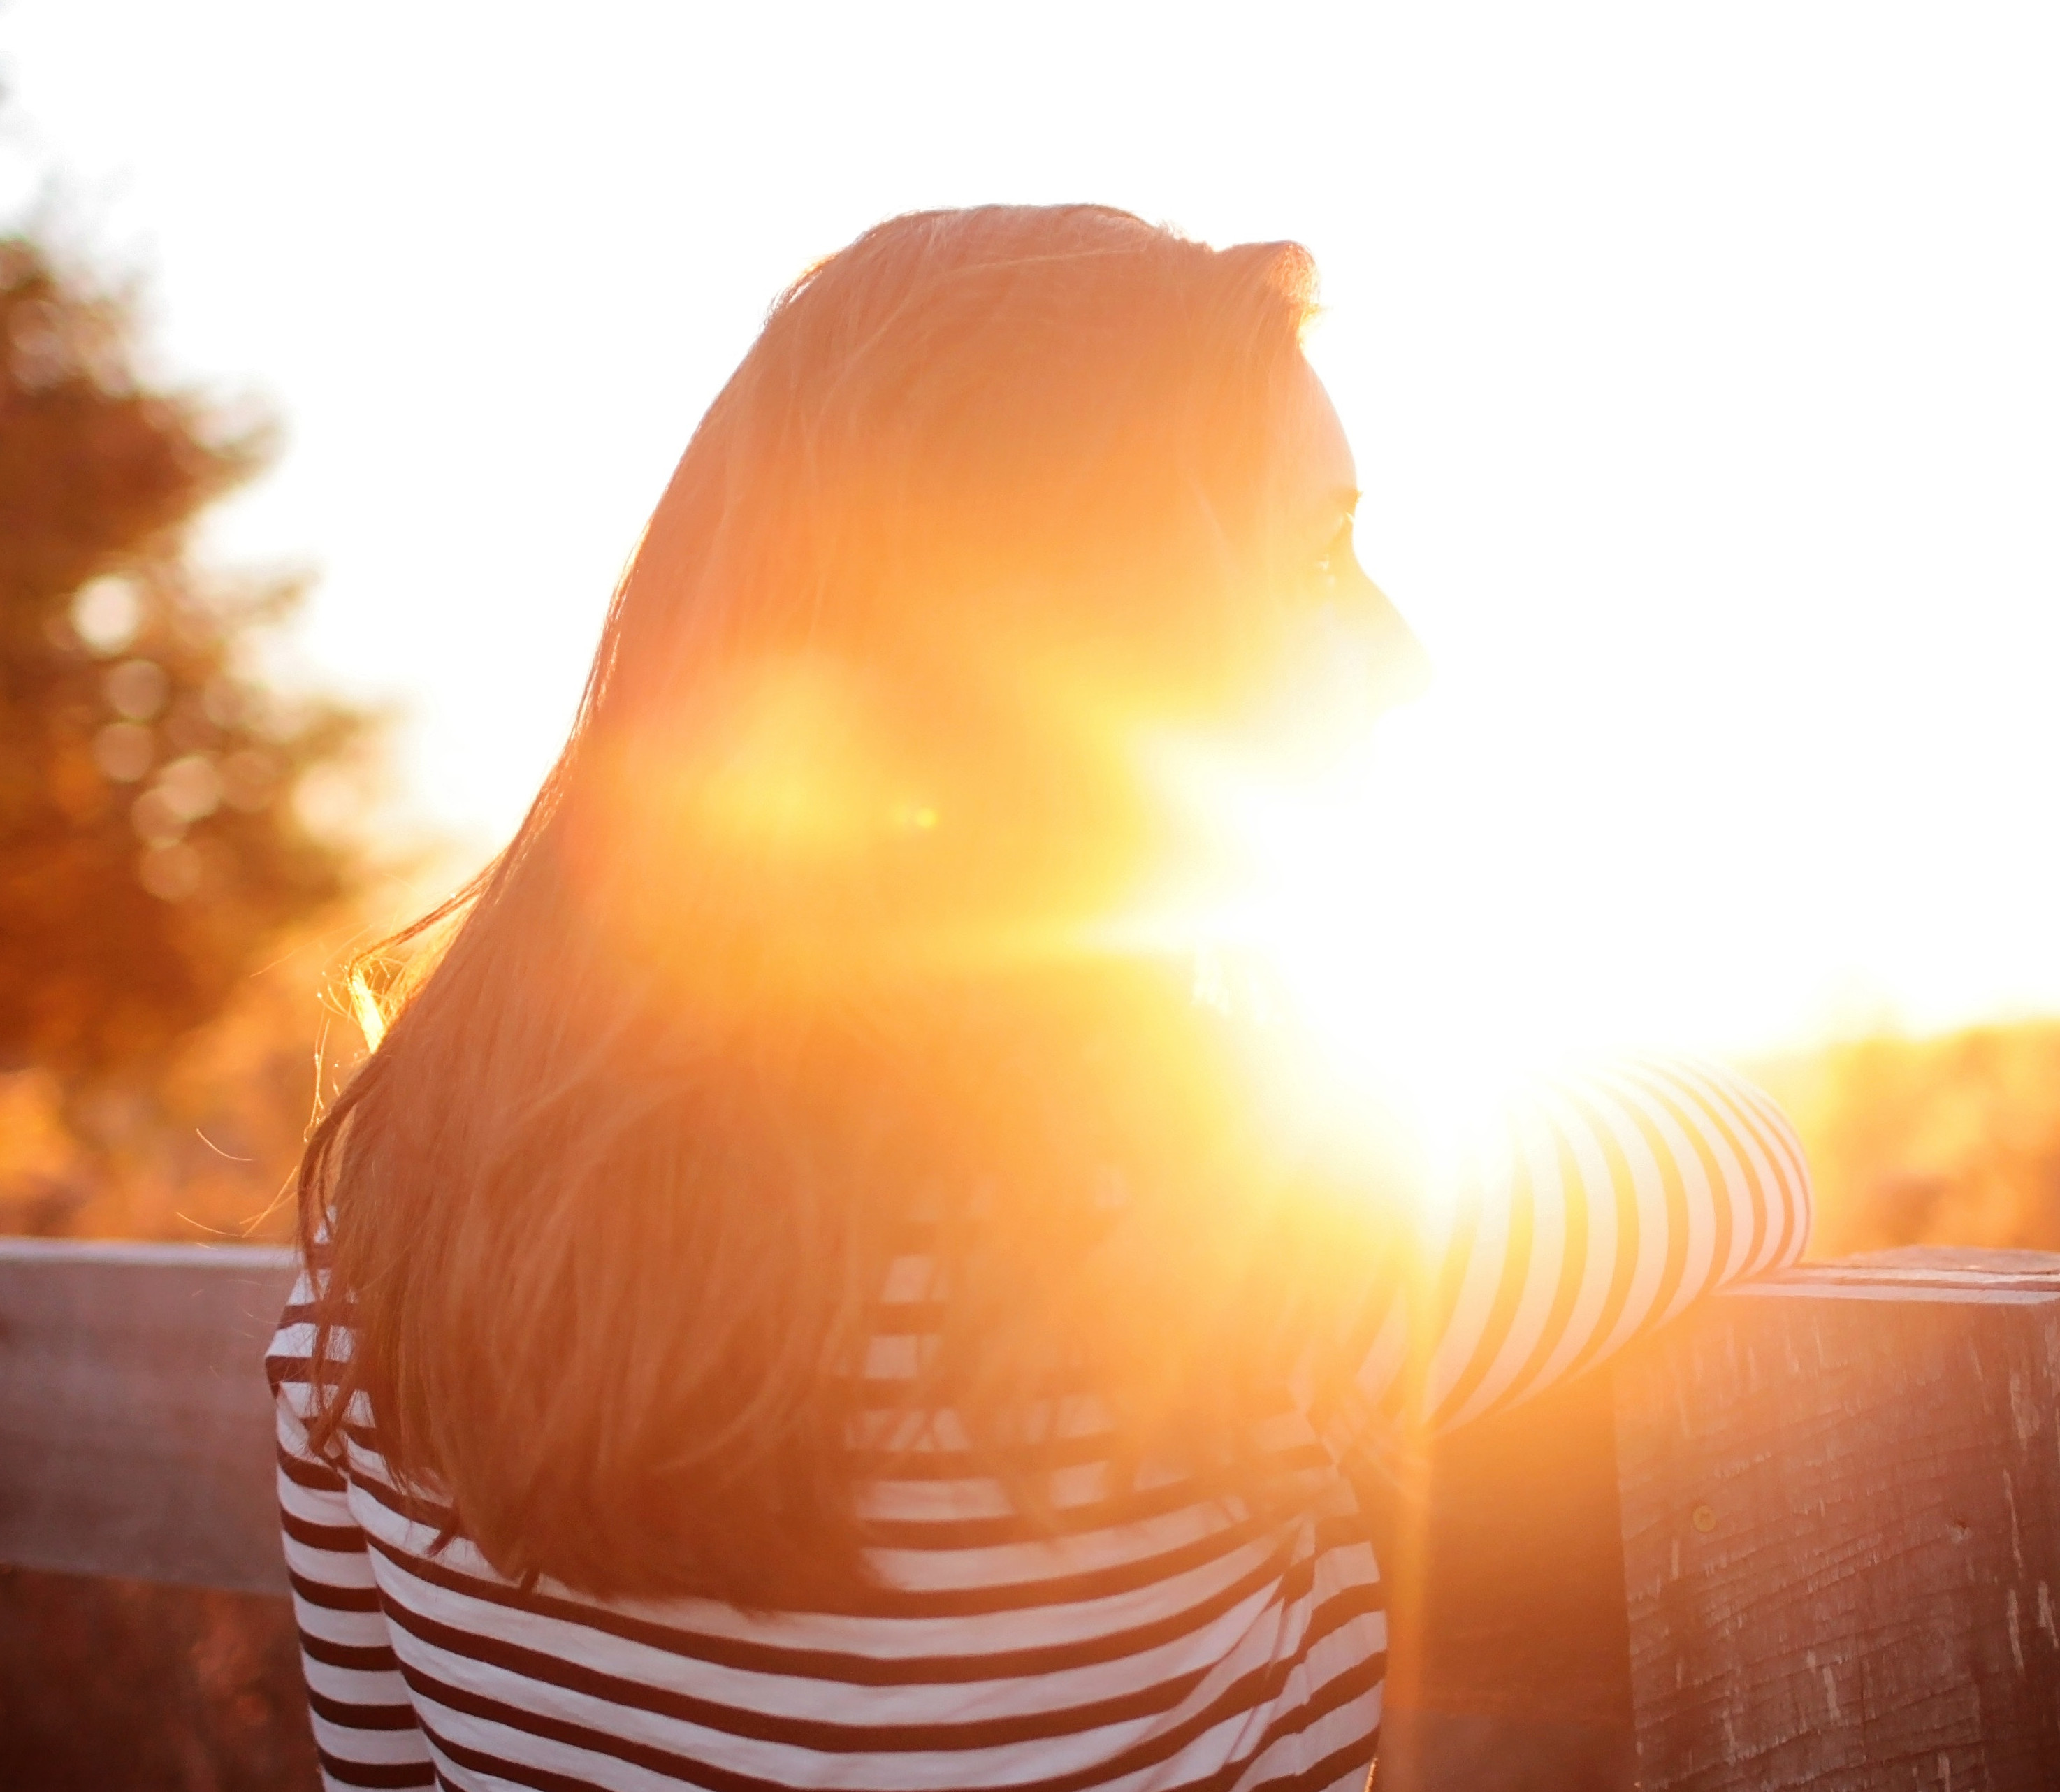
\includegraphics[width=0.5\textwidth]{exposure_example}
\caption{High lighting values in a standard RGB image}
\label{rgb_example}
\end{figure}

\section{Model Performance}
It is not only important to assess the accuracy of the predicted lighting, but also the resource requirements. A model that produces rough approximations with a lower memory footprint and computation time is still valuable, especially in the field of AR. For this we assess the memory usage and average inference time for our validation set. Testing the model performance across different hardware configurations is beyond the scope of this project.
% -----------------------------------------------------------------------------

\chapter{Conclusion}
\label{chap:conclusion}
We have presented a CNN approach for estimating the lighting at an object that exploits multiple views.
{\bf A compulsory chapter,     of roughly $5$ pages} 
\vspace{1cm} 

\noindent
\section{Achievements}
\section{Future Work}
\subsection{Full Scene Inference}
\subsection{Texture Resilient Inference}
\subsection{Video Inference}
\subsection{Spatial Lighting}
Talk about light fields!
%The concluding chapter of a dissertation is often underutilised because it 
%is too often left too close to the deadline: it is important to allocation
%enough attention.  Ideally, the chapter will consist of three parts:

%\begin{enumerate}
%\item (Re)summarise the main contributions and achievements, in essence
%      summing up the content.
%\item Clearly state the current project status (e.g., ``X is working, Y 
%      is not'') and evaluate what has been achieved with respect to the 
%      initial aims and objectives (e.g., ``I completed aim X outlined 
%      previously, the evidence for this is within Chapter Y'').  There 
%      is no problem including aims which were not completed, but it is 
%      important to evaluate and/or justify why this is the case.
%\item Outline any open problems or future plans.  Rather than treat this
%      only as an exercise in what you {\em could} have done given more 
%      time, try to focus on any unexplored options or interesting outcomes
%      (e.g., ``my experiment for X gave counter-intuitive results, this 
%      could be because Y and would form an interesting area for further 
%      study'' or ``users found feature Z of my software difficult to use,
%      which is obvious in hindsight but not during at design stage; to 
%      resolve this, I could clearly apply the technique of Smith [7]'').
%\end{enumerate}

% =============================================================================

% Finally, after the main matter, the back matter is specified.  This is
% typically populated with just the bibliography.  LaTeX deals with these
% in one of two ways, namely
%
% - inline, which roughly means the author specifies entries using the 
%   \bibitem macro and typesets them manually, or
% - using BiBTeX, which means entries are contained in a separate file
%   (which is essentially a databased) then inported; this is the 
%   approach used below, with the databased being dissertation.bib.
%
% Either way, the each entry has a key (or identifier) which can be used
% in the main matter to cite it, e.g., \cite{X}, \cite[Chapter 2}{Y}.

\backmatter

% -----------------------------------------------------------------------------

% The dissertation concludes with a set of (optional) appendicies; these are 
% the same as chapters in a sense, but once signaled as being appendicies via
% the associated macro, LaTeX manages them appropriatly.

\appendix

\chapter{An Example Appendix}
\label{appx:example}

%Content which is not central to, but may enhance the dissertation can be 
%included in one or more appendices; examples include, but are not limited
%to

%\begin{itemize}
%\item lengthy mathematical proofs, numerical or graphical results which 
%      are summarised in the main body,
%\item sample or example calculations, 
%      and
%\item results of user studies or questionnaires.
%\end{itemize}

%\noindent
%Note that in line with most research conferences, the marking panel is not
%obliged to read such appendices.

% =============================================================================

\end{document}
